% Candidate source: src-22a421a422f050bc84accae7bf41feb6903c62df04bd83f34d8267d28f49ee2e
% Source PDF SHA-256: 092e8e90dc1430ab2fa8b8ce79e072e317559e6bef29f1cb7461e9423925ec31
% PDF page 1 (printed page 262), question 11. The two printed sketches are identical.
% Redraw preserves visible/hidden linework; labels do not define drawing scale.
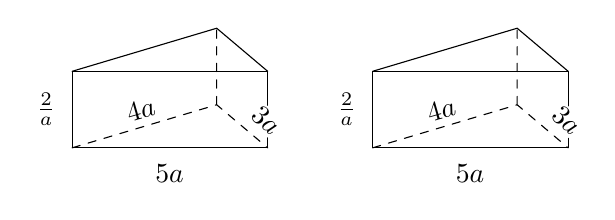
\begin{tikzpicture}[scale=0.72,line cap=round,line join=round]
  \foreach \shift in {0,5.3} {
    \begin{scope}[shift={(\shift,0)}]
      \coordinate (A) at (0,0);
      \coordinate (B) at (3.45,0);
      \coordinate (C) at (2.55,0.76);
      \coordinate (Aone) at (0,1.35);
      \coordinate (Bone) at (3.45,1.35);
      \coordinate (Cone) at (2.55,2.11);

      % Front rectangle and visible upper outline.
      \draw (A)--(B)--(Bone)--(Aone)--cycle;
      \draw (Aone)--(Cone)--(Bone);

      % Hidden base edges and rear vertical edge.
      \draw[dashed] (A)--(C)--(B) (C)--(Cone);

      \node[left] at (-0.12,0.68) {$\frac{2}{a}$};
      \node[below] at (1.72,-0.12) {$5a$};
      \node[above,rotate=16,fill=white,inner sep=1pt] at (1.27,0.46) {$4a$};
      \node[above right,rotate=-42,fill=white,inner sep=1pt] at (3.05,0.53) {$3a$};
    \end{scope}
  }
\end{tikzpicture}
